\section{Monday, 29 October 2018}

\subsection{Steps}
\begin{itemize}
\item We have analysed and interpreted the K-means groups and the outliers.
\item To achieve the previous point, we have grouped data by  ``\textit{labels}'' column and the columns with \texttt{X, Y, Z} contains the average of all data of distinct groups.  \\
To know what rows from the original dataset are outliers, we have added ``\textit{labels}'' column to the dataset. This column contains a ``$-1$'' value if the row is an outlier. We have filtered the rows which had a ``$-1$'' value in the ``\textit{labels}'' column and we have obtained the outliers.
\item He have plotted both interpreted results, the k-means groups and the outliers in a 3D graphic, using the original dataset. In this graphic (see Figure \ref{fig:outliers}), we can see where are the outlier points with regard to the other points of the dataset. 

\begin{figure}[!htb]
\centering
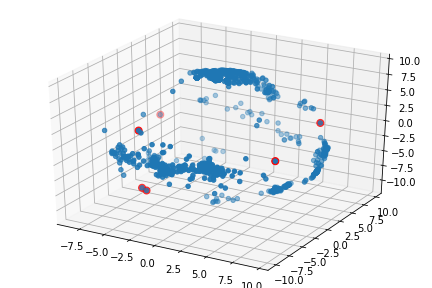
\includegraphics[width=0.5\textwidth]{../../reports/figures/outliers3D_AccelerometerStat.png}
\caption{The outlier points are shown in red color. The blue points are all the other dataset points}
\label{fig:outliers}
\end{figure}

\end{itemize}